\chapter{Tools And Scripts}
\thispagestyle{fancy}  % Use plain style for the first page of the chapter


















\section{mmorpdnd.py}

\subsection{Purpose}

This script serves as the backbone for an array of automatic linking and logistical features within MMORPDND. These functionalities typically operate on all files, encompassing crucial elements such as the generation of directories, HTML index files at the directory summits, establishment of uniform headers and navigation for all HTML documents, seamless interlinking between files, refinement of both HTML and CSS code, and an array of additional capabilities. When ran, this script will perform the following actions in the following order:

\begin{enumerate}
	\item Create Directory Structures if not already existing.
	\item Create index files for each directory.
	\item Update each index file to link to all files and images within the directory.
	\item Update the headers of all HTML files to the template HTML header.
	\item Update the navigation of all HTML files to the template navigation HTML.
	\item Search for invalid hyperlinks in HTML files and removes them.
	\item Search and hyperlink all words found in all HTML files to the appropriate HTML file whose name matches the words found.
	\item Beautify the code.
	\item Publicize the HTML files specified in the templates/lists/public\_files.list file.
\end{enumerate}






\subsection{Features}

\subsubsection{Create And Update index.html Files}

TODO

\subsubsection{Update All HTML Navigation And Headers}

TODO

\subsubsection{Update All HTML Hyperlinks}

TODO

\subsubsection{Beautify Files}

This feature will take all css and HTML files and `beautify' them. This is done by the BeautifulSoup Python library and will format all the files in a similar manner. Because this feature exists, the formatting of the HTML files when editing them is not needed, as it will be overwridden.   

\subsubsection{Publicize Files}

In some cases, links to a page may be desired for the players to access. In these cases, it is desired to remove the navigation header on the HTML pages as well as links to other pages within the MMORPDND database. This feature will facilitate doing just this. It is a simple feature to create pages for `public' (meaning links that the players in a campaign can access without linking them to the rest of the database) release. The script takes an input file called `templates/lists/public\_files.list'. The script will create duplicate files of all files listed in the `public\_files.list' with an appended `\_public' label on the file names. It will then parse all the public files and remove all links within the files that are not links to other public files. If a public file exists for one of the links, the link will instead be updated to the appropriate public file. 

The publicize files feature was originally it's own standalone script that was later integrated into the `mmorpdnd.py' script. This feature uses the `templates/lists/public\_files.list' file as input. This file should have relative file paths to all files that are wished to be made public (relative to the `mmorpdnd.py' script. The script will begin by creating a copy of all files (specified in the list file) with an appended `\_public' attached to the file name. These public files will have all header navigation data removed, and all links removed. In the case that a public file exists for what was previously linked to, the link will be updated to the public file rather than removed.










\subsection{Use}

The mmorpdnd.py script can be ran as a gui window or using the command line options. The two main features are `test' and `update'. The `test' feature will create fake files and then perform the update command on them. This is useful for testing if the features and newly added features are working properly. The `update' feature will perform a combination of tasks which updates all appropriate files to do the steps mentioned in the list above.

\subsubsection{GUI}

\begin{figure}[h]
	\centering
	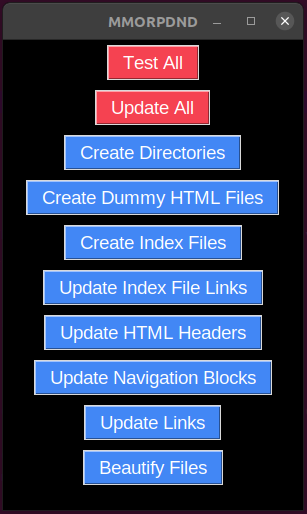
\includegraphics[width=0.5\textwidth]{images/mmorpdnd_gui.png}
	\caption{The MMORPDND Main GUI}
	\label{fig:mmorpdnd_gui}
\end{figure}

The GUI window is somewhat self explanatory. The two main features are represented by red buttons - the `test` and `update` features. There are also other buttons to simple perform and of the individual tasks using the appropriately associated button.

\subsubsection{Command Line}

The MMORPDND application supports some command line features. The update feature will run the updates for all HTML files.

\begin{lstlisting}
usage: mmorpdnd.py [-h] [-t] [-u] [-r]

MMORPDND Tools and apps.

options:
  -h, --help    show this help message and exit
  -t, --test    Runs the test-all feature then exits.
  -u, --update  Runs the update_all feature then exits.
  -r, --remove  Runs the remove_broken_links feature then exits.
\end{lstlisting}

















\section{templates/creator.py}



\subsection{Purpose}

The creator tool is a practical solution for converting basic template text files into functional HTML pages. It takes care of the technical aspects by automatically creating HTML files and filling in missing details, like character stats or other content. The tool understands the structure of your template files, recognizes placeholders, and replaces them with accurate data. Whether you're building character profiles, story summaries, or any content with consistent formatting, this tool ensures your HTML documents are correctly formatted and ready for use. It simplifies the process, letting you focus on content creation while it handles the conversion from templates to HTML.

\subsection{Use}

The creator tool is a powerful tool that contains many subtle features. It is important to understand these subtleties before using the tool and therefore I encourage the reader to read this enture section before use. 

\subsubsection{GUI}

\begin{figure}[h]
	\centering
	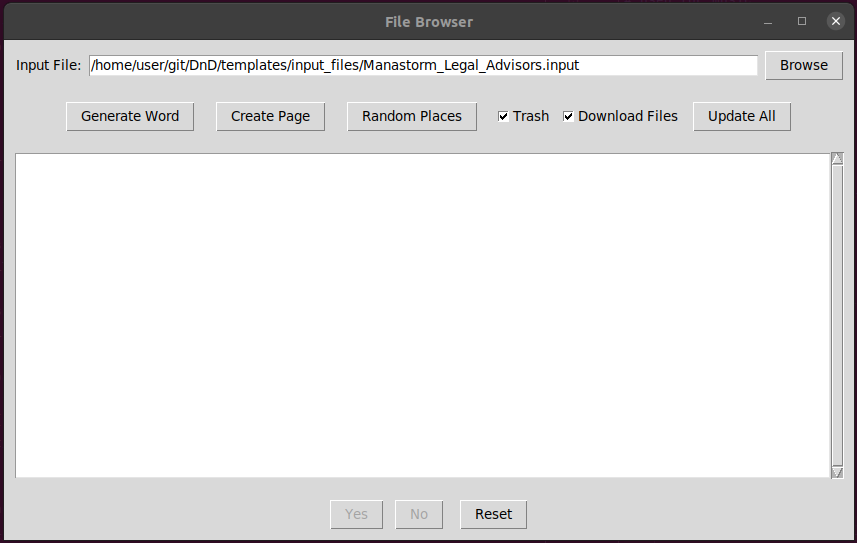
\includegraphics[width=0.9\textwidth]{images/creator_gui.png}
	\caption{The MMORPDND Main GUI}
	\label{fig:creator_gui}
\end{figure}

The main GUI of the creator tool has a few components. These include text boxes, buttons, and check boxes. 

The ``Input File" text box field is used to specify the input file that is to be processed by the tool. This file can be an `.input', `.char' or `.names' file. Ensure the file is in the proper format (see below sections) or unexpected behavior may occur. The `Browse' button is used to open a file explorer window for selecting a file and will automatically populate the ``Input File" text field when a file is selected. The large text box in the center of the GUI is where output generated from the tool as well as status messages are displayed.

The ``Generate Word" button is used for random word generation. This feature takes a list of words (whether names, places, or other) and generates a similar random word using the data in the input `.names' file. This is explained in more detail later in section \ref{section .names}. The ``Create Page'' button is used to generate an HTML file based on a `.input' or `.char' file and is explained in more details in the following sections. the ``Random Places'' file is used to generate place names based on an input `.names' file along with a `.list' file. These are explained mroe in later sections. The ``Yes", ``No", and ``Reset" buttons are used when user input is asked for. The ``Update All" button performs the same functions as the mmorpdnd.py update function (see the previous sections).

The ``Trash" checkbox will determine if processed files will be moved to the trash folder after processing and if duplicate files are to be deleted. Typically, the user will want this to be checked, but it is useful to leave unchecked for testing and if files will be processed multiple times. The ``Download Files" button determines if music files should be downloaded when `.input' files containing a dnd-music section are processed (this is explained mroe in later sections).

\subsubsection{Input Files (.input) \label{input files section}}

The input files are essentially just text files with the file extension `.input'. The main feature of the creator.py tool is to read in these input files, parse them, and generate the appropriate HTML files from them. These input files must follow a strict formatting but offer a few various helpful features. The name and main heading of the generated HTML file will be created based on the name of the input file (underscores will be replaced by spaces for the heading). Each line of the input file represents a 'section' of the HTML file that will be generated. Each line follows the following format:
\begin{lstlisting}
Heading Text[type]=Information text
\end{lstlisting}
The "Heading Text" is what will appear as the header for that HTML section. The "type" value is what determines the properties of this section and how it is interpreted by the creator tool. The "Information text" is the actual information for that section. The only exception to this rule is the first line which defines the "folder" that the HTML file generated from the input file will be placed into. This "folder" line is special in that it has no type and the creator tool will recognize the folder keyword and store this information separately. This folder line must be formatted as follows:
\begin{lstlisting}
folder=path/to/where/I/want/my/generated/file
\end{lstlisting}
The various types determine the formatting and decoding of the input file, and each type has small subtleties. The various types are
\begin{enumerate}
	\item dnd-image: This type is used to display an image or multiple images.
 	\item dnd-list: This is used to display a list of items.
 	\item dnd-info: This is used for general information and sections. It also supports listing information between paragraphs.
  	\item dnd-music: This is a section for storing various music for the regions.
\end{enumerate}

\subsubsection{dnd-image type}

The \textbf{dnd-image} type is used to display images specific to the file. The information text must contain three parameters separated by a semi-colon delimeter. These parameters are \textbf{img/image-name.jpg;image source;image caption}. The first parameter is simply the location of the image and the image name. These are typically placed in `templates/img'. The second is the source of the image, this is simply a string but is there to keep all images properly sourced. The third is a caption that will be displayed with an image. This caption is also a string and can be whatever the user desires. As an example, here's a proper dnd-image block (see figure \ref{fig:dnd-image-fig}):

\begin{lstlisting}
Coconatus Marmotta[dnd-image]=img/coconatus_marmotta.jpg;Created by Bing AI image creator;Coconatus Marmotta.
\end{lstlisting}

\begin{figure}[h]
	\centering
	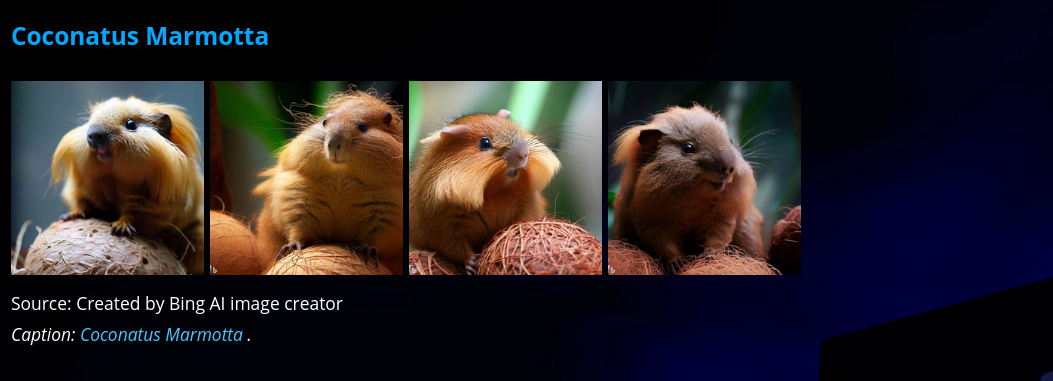
\includegraphics[width=0.8\textwidth]{images/dnd-image-section.png}
	\caption{A dnd-image section generated using 4 images.}
	\label{fig:dnd-image-fig}
\end{figure}

One unique feature of this is that if the image name does not exist (i.e. `img/coconatus\_marmotta.jpg'), the tool will append a ` (1)' to the name and search again (i.e. `img/coconatus\_marmotta (1).jpg'). If this new name is found, the tool will search for image names with the index incremented and include all such images (i.e. `img/coconatus\_marmotta (2).jpg', `img/coconatus\_marmotta (3).jpg', etc) in the output HTML block.  

\subsubsection{dnd-list type}

The \textbf{dnd-list} type is used to display a simple list of items. The information text must contain one or more parameters separated by a semi-colon delimeter. As an example, here's a proper dnd-list block (see figure \ref{fig:dnd-list-fig}):

\begin{lstlisting}
Landmarks and Other Features[dnd-list]=Talleril: A small island far off the coast of Alderpine.;Enthilma: A small island off the coast of Alderpine.;Lomelindei: The large world tree deep within Alderpine.
\end{lstlisting}

\begin{figure}[h]
	\centering
	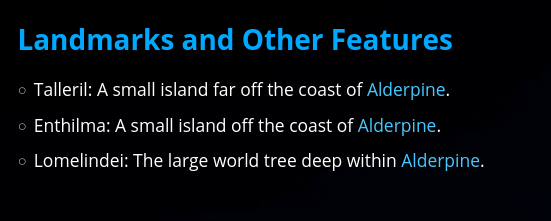
\includegraphics[width=0.6\textwidth]{images/dnd-list-section.png}
	\caption{A dnd-list section.}
	\label{fig:dnd-list-fig}
\end{figure}

\subsubsection{dnd-info type}

The \textbf{dnd-info} type is used to display a section of text. The information text must contain one or more parameters separated by a delimeter. The delimeter for this type will define the format of the sections within this text. For writing normal paragraphs, simple use a semi-colon (`;') delimeter. The semi-colon delimeter will make the next parameter appear as a normal paragraph. As an example, here's a proper dnd-info block (see figure \ref{fig:dnd-info-fig-01}):

\begin{lstlisting}
Some Paragraphs[dnd-info]=This is a paragraph.;This is a second paragraph.;This is a third paragraph.;etc...
\end{lstlisting}

\begin{figure}[h]
	\centering
	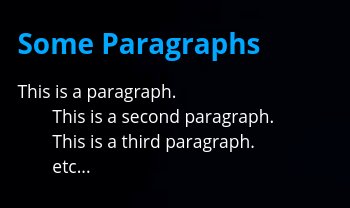
\includegraphics[width=0.6\textwidth]{images/dnd-info-section-01.png}
	\caption{A dnd-info section with only paragraphs. Note that the first paragraph will not be indented but all subsequent ones will be.}
	\label{fig:dnd-info-fig-1}
\end{figure}

To add in a list element between paragraphs, you can use a semi-colon and dash (`;-') delimeter. The `;-' delimeter will tell the creator tool that a list has began and the it will use all subsequential parameters with a preceeding `;-' delimeter as the list items until a different delimeter is entered or there is no more parameters to read in. As an example, here's a proper dnd-info block (see figure \ref{fig:dnd-info-fig-02}):

\begin{lstlisting}
Some Paragraphs and a List[dnd-info]=This is a paragraph.;-Here's a list item 1.;-Here's another list item;-Here's a third list item;Here's an ending paragraph.
\end{lstlisting}

\begin{figure}[h]
	\centering
	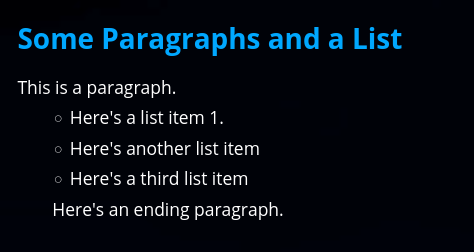
\includegraphics[width=0.6\textwidth]{images/dnd-info-section-02.png}
	\caption{A dnd-info section with a paragraph followed by a list, followed by a paragraph.}
	\label{fig:dnd-info-fig-2}
\end{figure}

To add a subsection, you can use the semi-colon followed by an asterik (`;*') as the delimeter. This delimeter has a somewhat special formatting in that there needs to be a second asterik to mark the end of the subsection heading. For example, `;*heading text*normal content text'. The `heading text' will display as a subheading, while the `normal content text' will be the main content under that subsection. As an example, here's a proper dnd-info block (see figure \ref{fig:dnd-info-fig-03}):

\begin{lstlisting}
Some subsections[dnd-info]=Here is a paragraph;*Subheading*Some text;Here's another paragraph;*Subheading 2*More text;Here's an ending paragraph.
\end{lstlisting}

\begin{figure}[h]
	\centering
	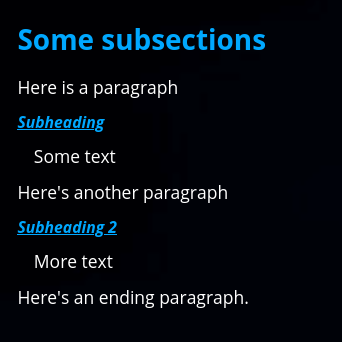
\includegraphics[width=0.6\textwidth]{images/dnd-info-section-03.png}
	\caption{A dnd-info section with some paragraphs and two subsections.}
	\label{fig:dnd-info-fig-3}
\end{figure}

\subsubsection{dnd-music type}

The \textbf{dnd-music} type is used to display a simple list of music items. The information text must contain one or more parameters separated by a semi-colon delimeter. Currently, this is primarily designed to work with youtube links. Given a simple youtube link, the code will find the name of the video and use that as the list information as well as keeping a link to the video itself. If the ``Download Links" checkbox in the GUI is enabled, the files will be downloaded as mp3 files and the folder next to the list item will be hyperlinked to the local file. These files will be located in a music folder. As an example, here's a proper dnd-music block using fake URL's (see figure \ref{fig:dnd-music-fig}):

\begin{lstlisting}
Music And Ambiance[dnd-music]=https://youtube_link_1;https://youtube_link_2;https://youtube_link_3
\end{lstlisting}

\begin{figure}[h]
	\centering
	
\includegraphics[width=0.6\textwidth]{images/dnd-music-section.png}
	\caption{A dnd-music section with two songs linked to.}
	\label{fig:dnd-music-fig}
\end{figure}


\subsubsection{dnd-table type}

The \textbf{dnd-table} type is used to display a simple table. The information text must contain one or more parameters separated by a semi-colon delimeter. The first parameter determines how many elements there are in each row. The rest of the parameters will then be parsed and placed into the table from left to right (top to bottom). As an example, here's a proper dnd-table block which creates a 3x2 table:

\begin{lstlisting}
Attributes[dnd-table]=3;Strength;10;+0;Dexterity;12;+1
\end{lstlisting}

\begin{figure}[h]
	\centering
	%\includegraphics[width=0.6\textwidth]{images/dnd-table-section.png}
	\caption{A dnd-table section with 3 columns and 2 rows.}
	\label{fig:dnd-table-fig}
\end{figure}


\subsubsection{Example Input File}

For example input files, you can look inside the templates/trash folder. This is where input files get placed after they are finished processing. The following is an example input file with an example of many different elements. The associated image files `foobar.jpg', `foobars (1).jpg' and `foobars (2).jpg' should be located in the templates/img folder for the below file to process correctly.

\begin{lstlisting}
folder=items

A Single Image[dnd-image]=img/foobar.jpg;Created by Someone;A foobar image.

Information Section[dnd-info]=Here is a paragraph of text.;Here is a second paragraph.

Information Section With Smaller Headers[dnd-info]=Here is a paragraph of text.;*Small Header* Here is a second paragraph.

A List Of Items[dnd-list]=item A; Item B; Item C; Item D

Multiple Images[dnd-image]=img/foobars.jpg;Created by Someone;Multiple foobar images.

Information Section with List[dnd-info]=Here is a paragraph of text followed by a list;-List_item_A;-List_item_B;-List_item_C;Followed by a paragraph.

Music And Ambiance[dnd-music]=https://youtube_link_1;https://youtube_link_2;https://youtube_link_3
\end{lstlisting}

The above file will create a file in the `items' folder found in `campaign/items'. The file will start with a header "A Single Image", where the foobar.jpg image is displayed. A caption of "A foobar image." will be under the image. Next will be a heading "Information Section" That has two paragraphs. Next a similar section with a header "Information Section With Smaller Headers", a paragraph, then a smaller header "Small Header", followed by another paragraph. Next, another heading "A List Of Items" with 4 items in the list. Following this, a "Multiple Images" heading with 2 images `foobars (1).jpg' and `foobars (2).jpg'\footnote{If an image is not found, it will automatically search for files with that image name with an appended (1), (2), (3),... If `(1)' is found, this image will be used and the number incrememted until no other images are found.} with a caption "Multiple foobar images." Next, another heading ``Information Section with List", with a paragraph, a list, and then another paragraph. Finally, a heading "Music And Ambiance" with links to three youtube videos. If the "download links" checkbox is enabled, these video's will be downloaded as mp3 files and the fodler icon will link to the local files.






\subsubsection{Character Files (.char)}

The character files are text files with the ".char" extension. These are a special type of input file that generates an HTML page specific for DnD character information. This was actually designed before the more general input file formatting outlined in the sections above and therefore lacks some of the versatility and extra features that can be included in the input files. Nevertheless, the character format creates an HTML page that should more than suffice for any npc characters and has many of its own unique features and capabilities. The .char file contains lines that define the various elements of a character. These lines to not currently support the types that are supported with the input files. Each line has a specific output format in the generated HTML file based on a template and the information itself. Some lines in the file are required while others are optional. The required lines must be present for the character file generated to be completed, while the optional lines will automatically be randomized and generated in the event that they are missing. Eahc line of the character file must be formatting in the following way:
\begin{lstlisting}
Keyword = Value
\end{lstlisting}
The "Keyword" is used by the creator tool to determine which type of information is being input, and the "Value" is the value of the information. For example "level = 3" would let the creator know that the character level is 3, and it will use that information appropriately.

Once the character file is appropriately filled out and created, it should be saved/placed in the templates/input\_files folder for processing by the creator tool just like the .input files. The creator tool will search the templates/img folder for any image references within the character files. This is different than the behavior of the input files (which rely on the user to specify the 'img' folder in the image path).






\subsubsection{Required Keywords}

The required keywords for a character file are the following:
\begin{enumerate}
	\item folder: This defines the folder that the output HTML character file will be placed. This should be a valid file path to a folder.
	\item name: This defines the name of the character.
	\item image: This is an image for the character. This should be just the image file name and extension (no path) and the image itself should be placed in the "templates/img" folder for automatic detection.
	\item class: This defines the DnD class. This must be a valid class from the following list:
		\begin{multicols}{3}
		    \begin{itemize}
		        \item barbarian
		        \item bard
		        \item cleric
		        \item druid
		        \item fighter
		        \item monk
		        \item paladin
		        \item ranger
		        \item rogue
		        \item sorcerer
		        \item warlock
		        \item wizard
		    \end{itemize}
		\end{multicols}
	\item abilities: The abilities of the character. This field is a list and should be entered using a comma (`,') as the delimeter.
	\item equipment: The equipment of the character. This field is a list and should be entered using a comma (`,') as the delimeter.
	\item proficiencies: These are the proficiencies of the character. This field is a list and should be entered using a comma (`,') as the delimeter. The proficiency bonus will automatically be calculated based on level and applied to proficiencies.
	\item information: General information and description of the character.
\end{enumerate}

The above list of keywords are all required and if they are missing or ill-formatted, unexpected behavior can occur.






\subsubsection{Optional Keywords}

The optional keywords for a character file are the following:
\begin{enumerate}
	\item level: This is the level of the character. If the level is not defined, it will default to 1. This must be an integer.
	\item hp: This will be generated automatically if not included based on the character class, level, and constitution\footnote{The constitution value is automatically generated based on the character class and level if not included.} value.
	\item ac: The Armor class value.
	\item size: The size of the character.
	\item type: The type of the character (creature, humanoid, animal, etc)
	\item alignment: The alignment of the character.
	\item speed: The speed of the character.
	\item resistances: The resistances the character has (if any).
	\item immunities: The immunities the character has (if any)
	\item senses: The senses. A ", Passive Perception: \#" will automatically be appended to this value based on a calculated passive perception.
	\item languages: Languages of the character.
	\item race: The race of the character.
	\item background: The background of the character.
	\item strength: This represents the character's physical strength and ability to exert force. This must be an integer.
	\item dexterity: This represents the character's agility, reflexes, and fine motor skills. This must be an integer.
	\item constitution: This measures the character's health, stamina, and resistance to illness and fatigue. This must be an integer.
	\item intelligence: This reflects the character's mental acuity, memory, and problem-solving skills. This must be an integer.
	\item wisdom: This represents the character's perception, intuition, and common sense. This must be an integer.
	\item charisma: This measures the character's charm, persuasion, and ability to influence others. This must be an integer.
	\item notes: Notes to add about the character that aren't contained in the `information' section.
\end{enumerate}

It is recommended to include all values in the character file and just use "None" for any string values that are not needed. This will prevent any un-expected bugs. Many of the values replace a string in a template file based on the values input, so if they are not specified, a correlated `search string' will appear in the final HTML file that serves as a placeholder for the information.






\subsubsection{Example Character File}

For example character files, you can look inside the templates/trash/chars folder. This is where input files get placed after they are finished processing. The following is an example character file. The associated image file foobar.jpg should be located in the templates/img folder for the below file to process correctly.

\begin{lstlisting}
folder = characters/player
name = fooBar
ac = 16 (natural armor)
hp = 84
level = 13
size = small
type = humanoid
alignment = neutral good
speed = 30 ft.
resistances = None
immunities = None
senses = Darkvision 60ft
languages = Common, Elvish
image = foobar.jpg
race = Fooling
class = wizard
background = Barber
strength = 15
dexterity = 13
constitution = 18
intelligence = 22
wisdom = 4
charisma = 14
abilities = basic attack: A basic attack with nothing special; prestidigitation
equipment = torch; small sword, a potato
proficiencies = strength, acrobatics, history
information = This is some info for foobar, the template character.
notes = No notes needed for template dude.
\end{lstlisting}

Once created, the file should be placed in the templates/input\_files folder and then processed via the creator.py tool.



\subsubsection{Optional Appended Input Types}

The character files can have optional input file type (specified in section \ref{input files section}) blocks specified after the normal character file information. This will generate sections identical to that of the input files at the bottom of the character file page. See the example below:

\begin{lstlisting}
... # other character stats here
proficiencies = strength, acrobatics, history
information = This is some info for foobar, the template character.
notes = No notes needed for template dude.

A new section[dnd-info]=Some more information.

Some more images[dnd-image]=img/images.jpg;images;More images of this char.
\end{lstlisting}






\subsubsection{Name Files (.names) \label{section .names}}

The `.name' files are essentially lists of names to be used. The file extension `.names' is simply to differentiate between lists used as other things and lists that are specifically for name generation. These files should each have a common theme (i.e. a file for human names). Within the files, there should be one name per line. The ``Generate Word" button is used for random word generation. This feature takes a list of words (whether names, places, or other) in the form of a names file and generates a similar random word using the data in the input `.names' file. After generating a word, it will also ask the user if they would like to append that word to the list for future generation/use. 

The algorithm used to generate these names is quite straight forward and outlined in detail below. At first, AI name generation was thought of as an option, but this tended to give very cliche, repetitive, and similar sounding names - it wasn't very creative. The algorithm added here generates entirely new words that follow the patterns and structure of the words in the input lists. The more words that are contained in the names list, the better the name generation will be. With small lists, the name generation may not be that good.

The algorithm used for name generation begins by reading in all words in the names file. The words are sorted into a probability matrix that determines the probability of which letter should follow another based on all the occurrences of those letters within the words of the list. For example, the word `hello' would generate the below probability matrix.

\begin{lstlisting}
{
    "e": {
        "l": 1.0
    },
    "h": {
        "e": 1.0
    },
    "l": {
        "l": 0.5,
        "o": 0.5
    },
    "o": {}
}
\end{lstlisting}

Once generated, a small number of corrections and adjustments are made, and then this probability matrix is used to construct a new word. The length is randomized based on the smallest and largest words within the names file.





\subsubsection{List Files (.list) \label{section .list}}

The `.list' files are simple lists of information. These are similar to the `.names' files, with the difference that these list files are typically used internally within the various tools.













\subsubsection{Command Line}

The creator application supports limited command line features. The file option will run the creator for a single input file and then update all files.

\begin{lstlisting}
$ ./creator.py -h
usage: creator.py [-h] [-f FILE]

MMORPDND Creator Tool.

options:
  -h, --help            show this help message and exit
  -f FILE, --file FILE  Run the creator for a single input file and update all files.
\end{lstlisting}

















\section{templates/lists/check\_link\_validity.py}


This script will simply check the validity of the \textit{links.list} file.












\section{templates/lists/organize\_random\_places.py}

This script will sort the location names in the \textit{random\_place.names} file based on the last word in each item. The output will be saved to \textit{random\_place\_sorted.names} so that the original file will not be disturbed.














\section{templates/lists/remove\_duplicates.py}

This is a simple command line tool that will search through a file and remove any duplicate entries. This is useful when dealing with large name files or list files.

\begin{lstlisting}
usage: remove_duplicates.py [-h] [-f FILE] [-a]

Remove duplicate lines from files

optional arguments:
	-h, --help            show this help message and exit
	-f FILE, --file FILE  Path to the file
	-a, --all             Run against all files in the current folder
\end{lstlisting}














\section{templates/img/fix\_image\_extensions.py}

This tool will simply search through all files in the templates/img folder and replace all `.jpeg' extensions with `.jpg'. This is both for consistency and  functionality of the other apps.



















\section{templates/languages/translator.py}

This tool is still in development and not yet functioning.



















\section{templates/reset\_all\_files.py}

The `reset\_all\_files.py` script provides functions for restoring all files to a state where they are prepared to be processed by the `creator.py' application. It performs three main operations: copying image files to the `tempaltes/img' folder, deleting HTML files in the campaign directory structure, and moving specific input files back to the `templates/input\_files' folder. The script includes the following functions:

\begin{enumerate}
    \item \textbf{`copy\_images(source\_dir, dest\_dir)`:} This function copies image files from a specified source directory to a destination directory. It identifies images based on common file extensions such as `.png`, `.jpg`, `.jpeg`, and `.gif`. The function traverses the source directory and its subdirectories, specifically looking for folders named 'img', and copies the detected image files to the destination directory.

    \item \textbf{`delete\_html\_files(directory)`:} This function deletes all HTML files within a specified directory and its subdirectories. It traverses the directory tree, identifies files with a `.html` extension, and removes them. This is useful for cleaning up directories from unwanted HTML files.

    \item \textbf{`move\_input\_files(source\_dir, dest\_dir)`:} This function moves files with `.input` or `.char` extensions from a source directory to a destination directory. It ensures that the destination directory exists, creating it if necessary. The function traverses the source directory and moves the matching files to the destination directory.
\end{enumerate}

The script is configured with paths relative to its location:
\begin{itemize}
    \item The \texttt{campaign\_dir} points to the `../campaign` directory relative to the script directory.
    \item The \texttt{dest\_img\_dir} is set to the `img` directory within the script's directory for storing copied images.
    \item The \texttt{trash\_dir} is designated as the `trash` directory within the script's directory.
    \item The \texttt{input\_files\_dir} is set to the `input\_files` directory within the script's directory for moving input files.
\end{itemize}

The script performs the following operations when executed:
\begin{enumerate}
    \item Copies image files from the `campaign` and `trash` directories to the `img` directory.
    \item Deletes all HTML files from the `campaign` directory.
    \item Moves `.input` and `.char` files from the `trash` directory to the `input\_files` directory.
\end{enumerate}

Ensure that the directories specified (e.g., `campaign`, `img`, `trash`, `input\_files`) exist and are accessible. The script creates directories as needed but assumes the necessary permissions are available.

















\section{templates/stockpile/}

This directory contains the various elements of the Stockpile system (see \ref{S.T.O.C.K.P.I.L.E}).

\subsection{stockpile.py}

The stockpile.py script is the main application controlling the Stockpiles. The stockpile script takes an optional config file where the various parameters for stockpile updating and generation can be modified (see /ref{stockpile config}).

\begin{lstlisting}
usage: stockpile.py [-h] [-c CONFIG] -g GENERAL -t TRADE [-b BUY] [-s SELL] -o OUTPUT [-i]

S.T.O.C.K.P.I.L.E System Interface and Database Updater.

optional arguments:
	-h, --help            show this help message and exit
	-c CONFIG, --config CONFIG
	                    The config file containing key-value pairs representing configuration parameters, each line formatted as 'variable=value.'
	-g GENERAL, --general GENERAL
	                    The file containing general store items.
	-t TRADE, --trade TRADE
	                    The file containing random and trade items.
	-b BUY, --buy BUY     The file containing the buy price history of the various items. Including this option will update this.
	-s SELL, --sell SELL  The file containing the sell price history of the various items. Including this option will update this.
	-o OUTPUT, --output OUTPUT
	                    The output file to compare to and update. This should be a .input file with the lists formatted in the dnd-table format (see documentation).
	-i, --initial         Generates an initial .input file for processing.
\end{lstlisting}

\subsubsection{Item Lists}

The item lists are the master list that contains all of the general and specialty items for the Stockpiles. These lists are fed into the stockpile app with the `-g' and `-t' options. The lists should be formatted such that each line represents a single item. Each item will contain 3 parts separated by a semicolon delimiter - A name, a price, and a description (see below for example file). 

\begin{lstlisting}
Abacus;2g;2 lb.
Acid (vial);25g;1 lb.
Alchemist fire (flask);50g;1 lb.
Arrows (20);1g;1 lb.
Blowgun Needles (50);1g;1 lb.
Crossbow bolts (20);1g;1.5 lb.
Sling bullets (20);4c;1.5 lb.
Antitoxin (vial);50g;
Backpack;2g;5 lb.
\end{lstlisting}

The distinction between these two lists is in the types of items they contain. The general list should be easily obtainable and typically available items for an area. In contrast, the Trade/Specialty items are rare items, or things that may or may not be available - primarily carried by traders to a region.

\subsubsection{Buy and Sell Price History Lists \label{stockpile:buy and sell}}

The buy and sell price history files can start blank. The application will create these by adding items into the list that are not already found. The files are formatted so that each line represents a single item. The lines will contain a number of elements separated by a semi-colon delimiter. The first element is the item name. All later elements are the various prices of the items as they have changed (thus capturing the price history).

\begin{lstlisting}
Abacus;1.9;1.95;2.03;2.16;2.08;2.07;2.13;1.99;1.96;2.03;2.06;2.17;2.27;2.31
Acid (vial);27.32;26.57;28.75;28.61;28.42;28.7;28.01
Alchemist fire (flask);50.52;52.08;54.07;55.43;57.35
Alchemist supplies;48.03;46.5;45.58;47.4;45.4;44.22;42.28;40.12;40.93
Antitoxin (vial);55.09;54.65;57.01;58.46;61.02;64.23;68.13;68.74;66.47
Arrows (20);1.01;1.02;0.97;1.01;0.98
\end{lstlisting}

\subsubsection{Output list}

The output of the stockpile program will be a `.input' file that matches the correct format to display all items in a list. The file will have two sections, one for general items and one for specialty/trade items. See Figure \ref{fig:stockpile_general_list} for the example html file that is produced from an input file from the stockpile output.

\begin{figure}[h]
	\centering
	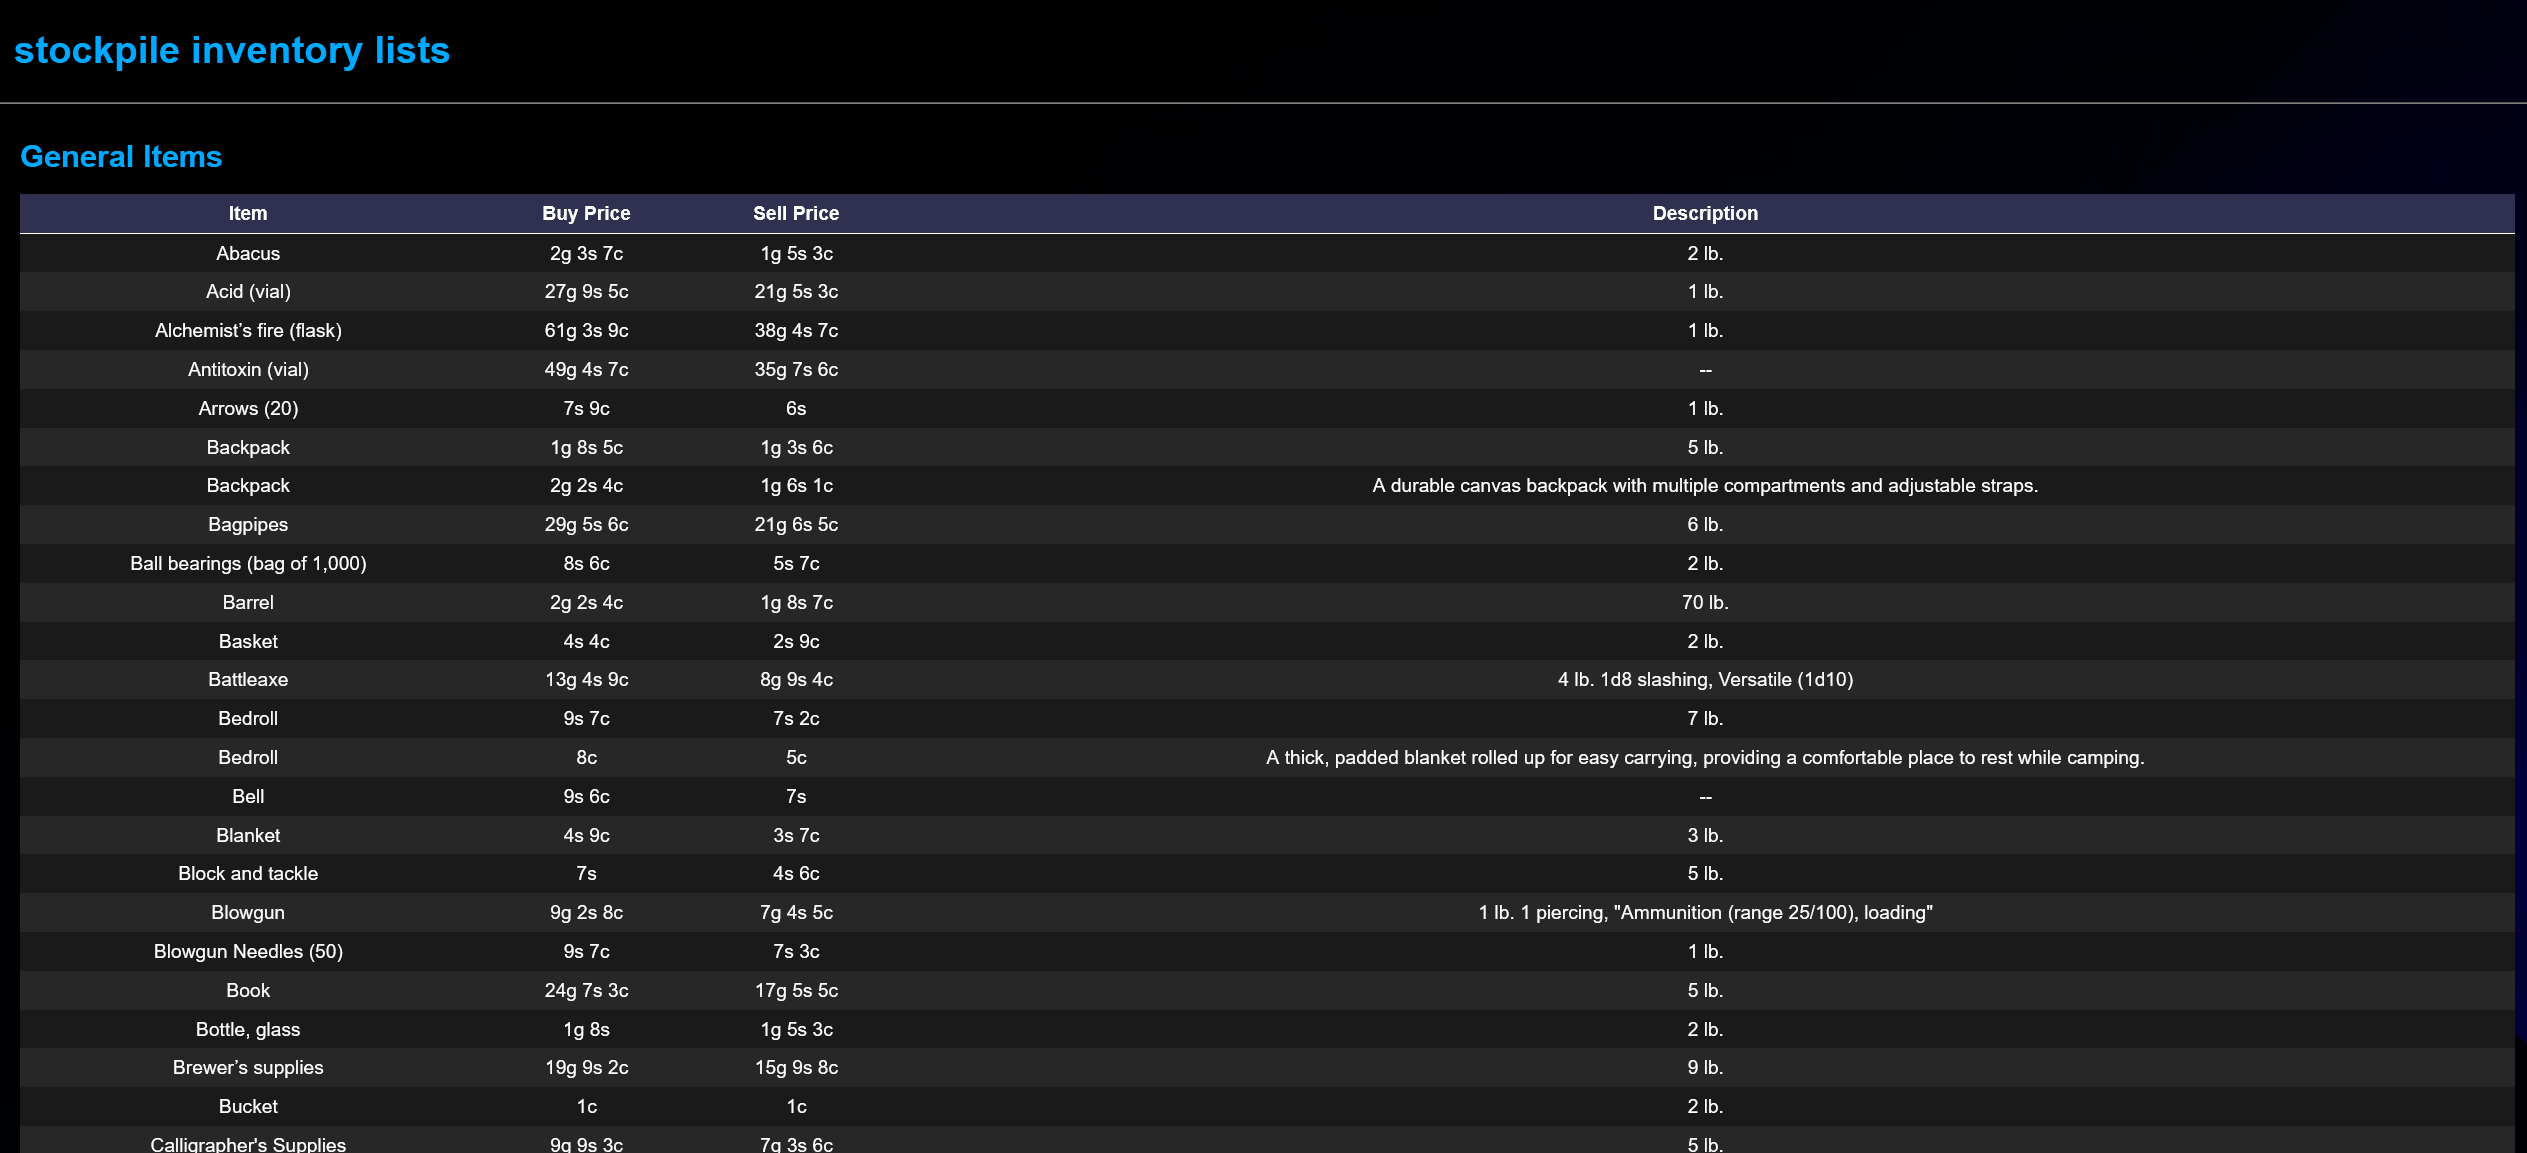
\includegraphics[width=\textwidth]{images/stockpile_general.png}
	\caption{A dnd-table generated by the stockpile output file.}
	\label{fig:stockpile_general_list}
\end{figure}

\subsection{Stockpile Config\label{stockpile config}}

The configuration file consists of key-value pairs, where each line follows the `variable=value' format. Below is a list of the available configuration parameters, their types, and descriptions.

\begin{itemize}
    \item \textbf{cadence (int)}: The frequency in seconds at which the configuration parameters are updated. Default: 86400.
    \item \textbf{general\_price\_variance (float)}: The variance factor for general item prices. Default: 0.05.
    \item \textbf{trade\_price\_variance (float)}: The variance factor for trade item prices. Default: 0.2.
    \item \textbf{general\_items\_percent\_in\_stock (float)}: The base percentage of general items that are in stock at any given time. Default: 0.9.
    \item \textbf{general\_items\_percent\_in\_stock\_variance (float)}: The variance on the \textit{general\_items\_percent\_in\_stock} value. Default: 0.05.
    \item \textbf{trade\_items\_percent\_in\_stock (float)}: The base percentage of trade items that are in stock at any given time. Default: 0.2.
    \item \textbf{trade\_items\_percent\_in\_stock\_variance (float)}: The variance on the \textit{trade\_items\_percent\_in\_stock} value. Default: 0.1.
    \item \textbf{sell\_price\_percentage (float)}: The base percentage of the buy price to determine sell prices for items. Default: 0.75.
    \item \textbf{sell\_price\_percentage\_variance (float)}: The variance of the sell prices. Default: 0.1.
    \item \textbf{general\_items\_input\_tag (str)}: The tags that appear as the header for the dnd-table lines in the .input files for general items. Default: "General Items".
    \item \textbf{trade\_items\_input\_tag (str)}: The tags that appear as the header for the dnd-table lines in the .input files for trade items. Default: "Specialty/Trade Items".
\end{itemize}

Below is an example of a configuration file with custom values:

\begin{lstlisting}
cadence=43200
general_price_variance=0.1
trade_price_variance=0.15
general_items_percent_in_stock=0.85
general_items_percent_in_stock_variance=0.04
trade_items_percent_in_stock=0.25
trade_items_percent_in_stock_variance=0.08
sell_price_percentage=0.7
sell_price_percentage_variance=0.15
general_items_input_tag=Basic Items
trade_items_input_tag=Trade Goods
\end{lstlisting}

When the application starts, it attempts to load the configuration parameters from the specified file. If no file is provided or the file is not found, default values are used, and a warning is displayed. If the configuration file is not found, the application will output an error message and continue using the default values. Ensure the file path is correct and the file is accessible. For constructing a configuration file, the application provides a help message detailing the available variables and their descriptions. Use the `variable=value' format.









\subsection{stockpile\_plot.py}

The `stockpile\_plot.py' script will create plots of all the buy and sell prices of the generated stockpile prices (see section \ref{stockpile:buy and sell}). The input files should be formatted by the stockpile.py script or match the format of the files output by that script.

\begin{lstlisting}
usage: stockpile_plot.py [-h] -b BUY -s SELL [-i ITEM] [-o OUTPUT]

S.T.O.C.K.P.I.L.E.S price history plotting.

optional arguments:
	-h, --help            show this help message and exit
	-b BUY, --buy BUY     The file containing buy price history for the stockpile items.
	-s SELL, --sell SELL  The file containing sell price history for the stockpile items.
	-i ITEM, --item ITEM  The item to search for and plot. This will display the plot as well. If not specified, all plots will be generated.
	-o OUTPUT, --output OUTPUT
	                    The folder to output all plots to. This option will be ignored if '-i' is specified.
\end{lstlisting}


\begin{figure}[h]
	\centering
	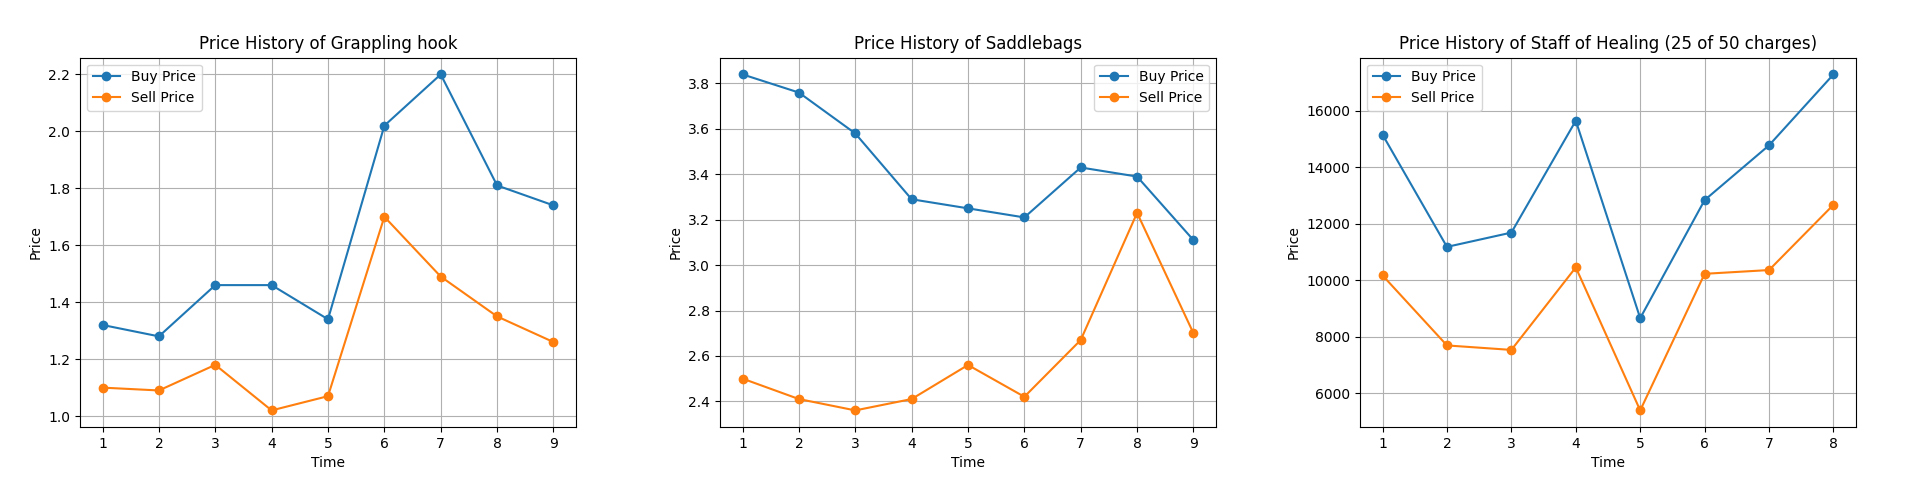
\includegraphics[width=\textwidth]{images/sample_plots.jpg}
	\caption{Three sample plots created by the stockpile\_plot.py script for the stockpile system.}
	\label{fig:sample_plots}
\end{figure}











\subsection{templates/add\_external\_links.py}

The `add\_external\_links.py' script processes HTML files to replace specified words with corresponding hyperlinks. It is designed to automate the embedding of links within a set of HTML files based on a predefined list. 

To use the script, ensure the list of words and links is saved in a file (e.g., lists/links.list), with each line formatted as `word,link'. Place the HTML files to be processed within the target directory (e.g., ../campaign) - which is the default place they should be. Then run the script. It will load the word-link pairs, find all HTML files in the specified directory, and replace the specified words in each HTML file with the corresponding hyperlinks (in the appropriate HTML format).










\subsection{templates/visualize\_nodes.py}

This script generates and visualizes a network graph of HTML files within a campaign (or a specified with some modification) directory. The script begins by defining the directory to scan for HTML files and then proceeds to build and visualize the graph. The process consists of the following steps:

\begin{enumerate}
    \item \textbf{Extracting Links:} The script uses the `extract\_links' function to parse HTML content and extract links to other HTML files. This function utilizes the BeautifulSoup library to find all anchor tags with an `href' attribute that ends with `.html'.
    
    \item \textbf{Building the Graph:} The `build\_graph' function constructs a directed graph using NetworkX. It scans the given directory and its subdirectories for HTML files, excluding `index.html' and files containing `\_public'. For each HTML file, the function adds a node to the graph and creates directed edges between nodes based on the links found in the files.
    
    \item \textbf{Visualizing the Graph:} The `visualize\_graph\_plotly' function visualizes the graph using Plotly. It computes the layout of the graph with `nx.spring\_layout' and generates traces for edges and nodes. The node sizes are dynamically adjusted based on their degree, and the final interactive visualization displays the network of HTML links.
\end{enumerate}

\begin{figure}[h]
	\centering
	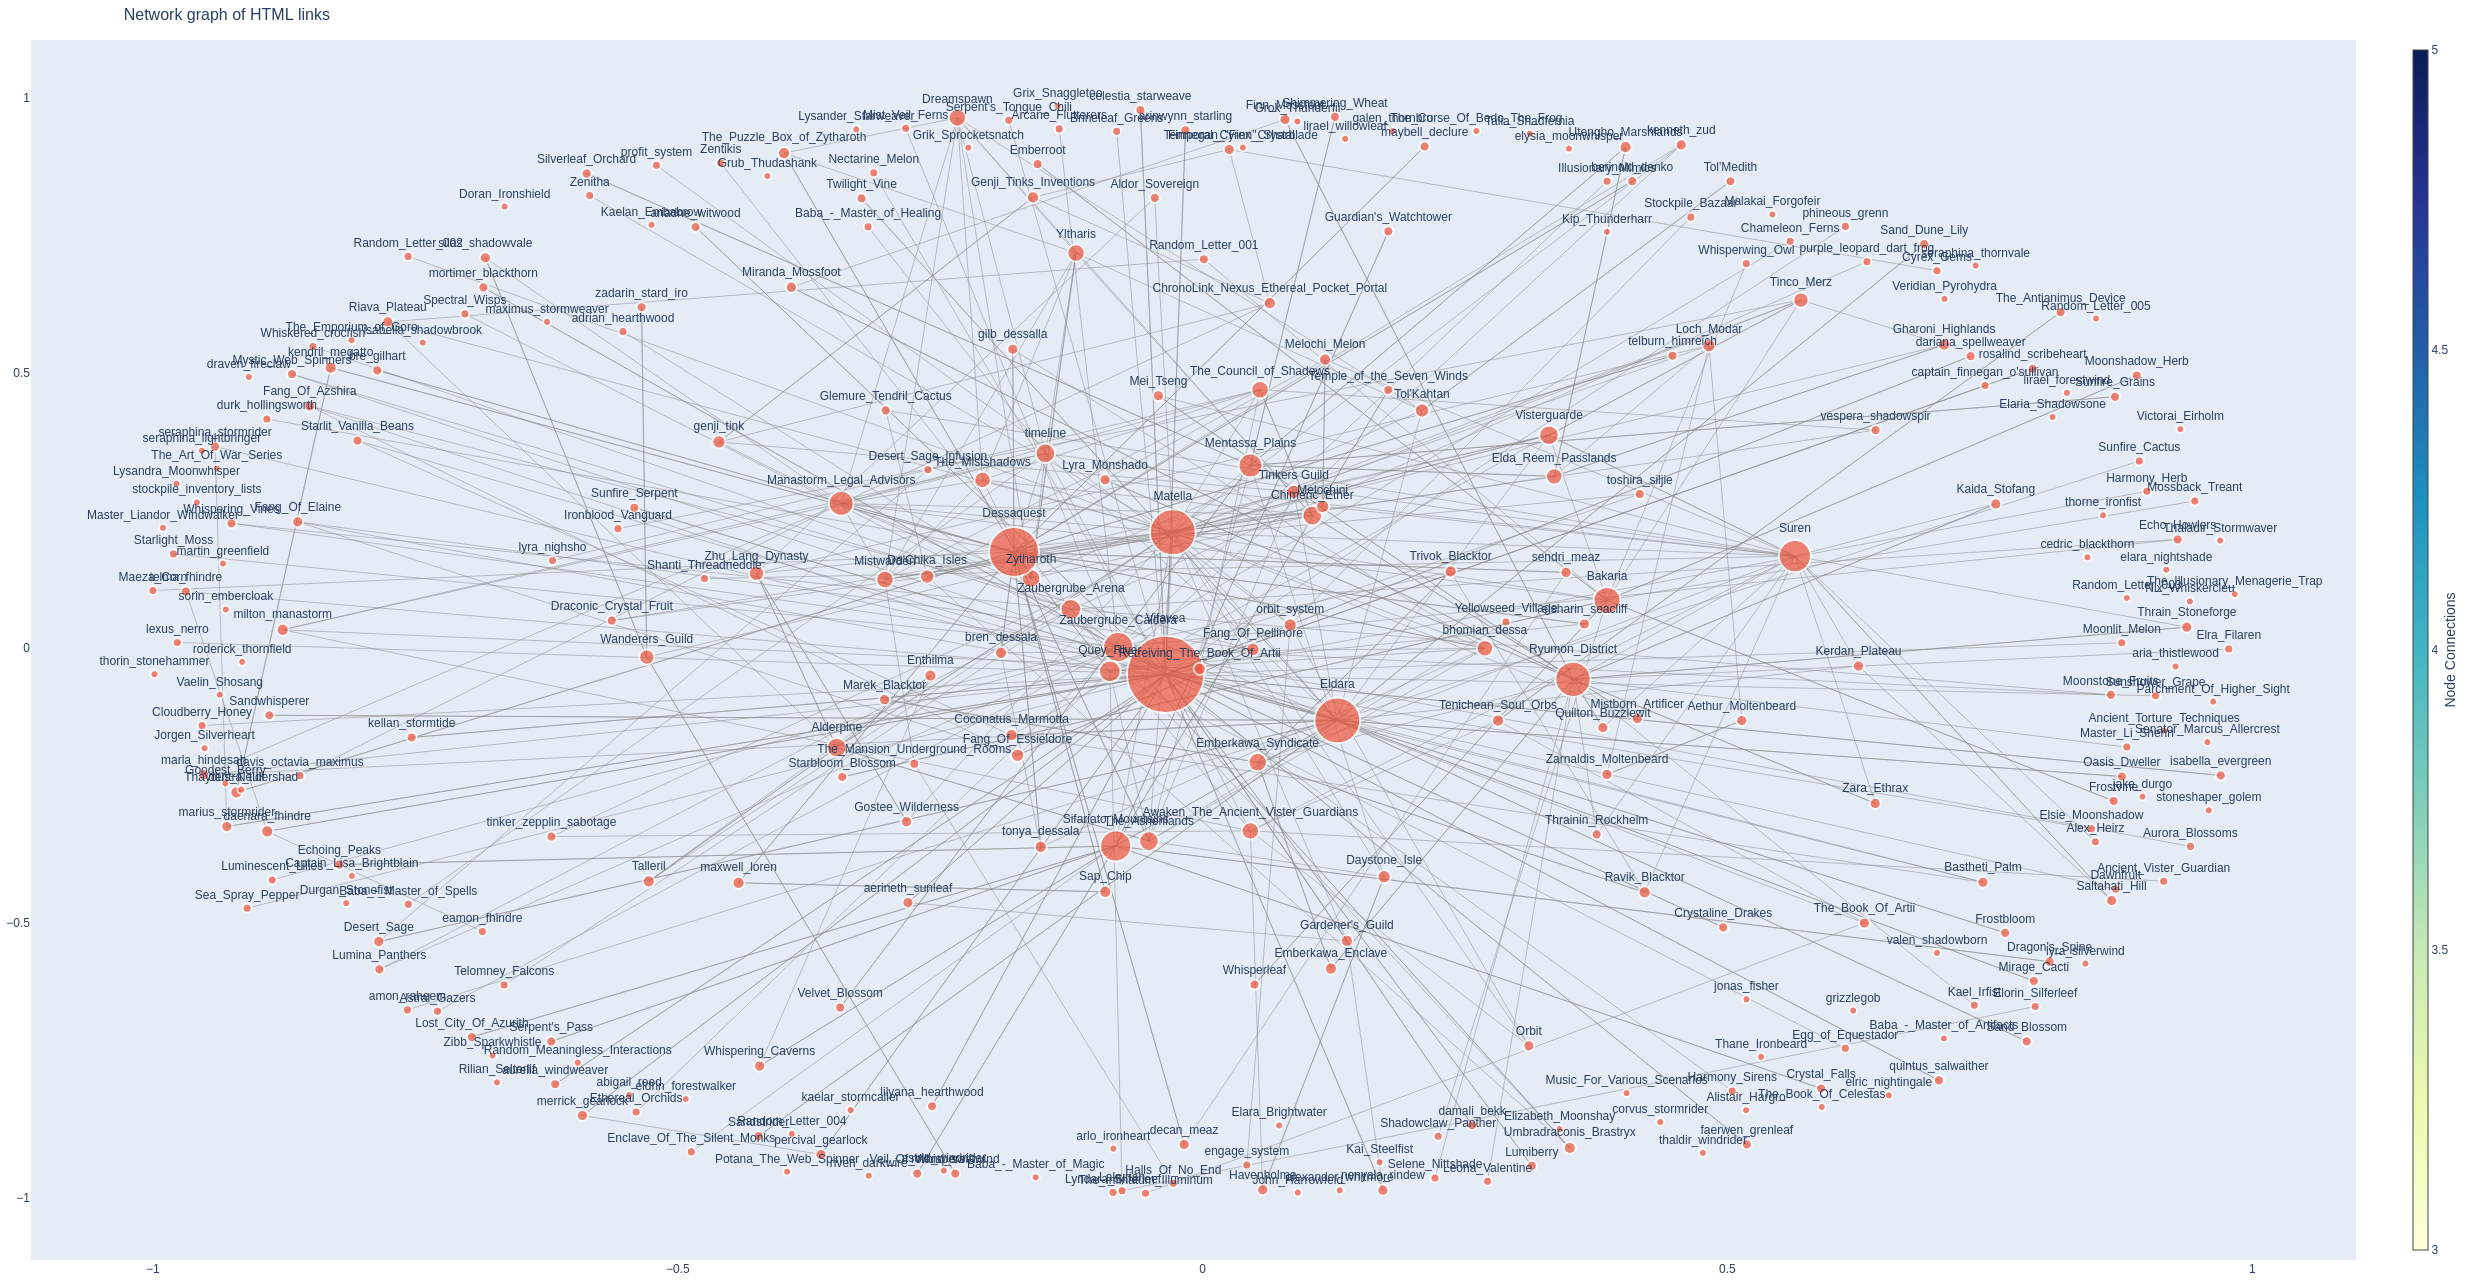
\includegraphics[width=\textwidth]{images/node_visualization.png}
	\caption{A visualization of the nodes for all HTML files and their connections. The larger nodes represent files that have more links within them.}
	\label{fig:node_visualization}
\end{figure}








\subsection{templates/trash/img/cleanup\_trash\_images.py}

This script is designed to identify and delete image files from the campaign (or a specified with some modification) directory if matching files are found in a database folder. The script starts by defining the current directory as the script folder and calculates the relative path for the campaign folder. It then proceeds to find and remove matching image files from the script folder. The script operates as follows:

\begin{enumerate}
    \item \textbf{Getting Image Files:} The script uses the `get\_image\_files' function to generate a list of image files from a given directory. It filters files based on common image file extensions including `.png', `.jpg', `.jpeg', `.gif', `.bmp', and `.tiff'.
    
    \item \textbf{Finding and Deleting Images:} The `find\_and\_delete\_images' function searches for images in the database folder that match the names of images found in the script folder. For each matching image file, it deletes the file from the script folder.
    
    \item \textbf{Execution:} The script sets the paths for the script folder and the database folder. It then calls the `find\_and\_delete\_images' function to perform the matching and deletion operation.
\end{enumerate}








